\documentclass[12pt]{article}
\usepackage[utf8]{inputenc}
\usepackage{graphicx}
\graphicspath{{images/}}
\begin{document}
\begin{center}
\huge\underline{``Emerging Technologies in Healthcare''}
\end{center}
\begin{center}
 
\includegraphics[scale=0.8]{nitlogo.png }
\end{center}
\vspace{1cm}
\begin{center}
   \emph{\large By}\\
\Large{Raj Motwani }\\
\large{Roll No- 21111042}\\
\large{Biomedical 1st Sem}\\
\end{center}
\clearpage
\section*{Emerging Technologies in Healthcare}
The healthcare sector of today benefits immensely from technological advancements. Emerging technologies are helping develop newer, better treatments while alleviating cost burdens. Some technologies are yet to be explored to their full potential, but have still brought about a massive shift in the sector. Innovations such as artificial intelligence and robotics are completely changing the landscape, ushering in a new future for healthcare.

Digitalization has sped up transformation in industries. Today, equipment and processes are benefiting from new technologies, which are increasing productivity and efficiency across sectors. The global healthcare sector has also gained from these emerging trends. While the adoption rate is still slow, it is a boon to patients and doctors alike.
Healthcare technologies are diverse and encompass devices, medicines, vaccines, procedures, and systems to streamline operations, trim costs, and improve the quality of care delivered. Artificial intelligence (AI), blockchain, robotics, bio-printing, and nanotechnology are among the most promising technologies in the healthcare space.
\subsection*{AI}
 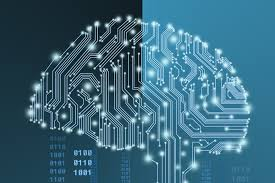
\includegraphics[scale=0.6]{ai.jpeg }
 \\
A greater adoption of AI can revolutionize the entire healthcare industry. AI usage within the healthcare industry was estimated to grow exponentially and investments in this space could reach USD 6.6 billion by 2021. AI can be applied in multiple, diverse ways—in operations to identify high-risk patients and also to automate medication reminders and dosages. For example, Google DeepMind Health is building AI tools that can analyze vast amounts of medical data to discover new, easy ways to detect and treat diseases. DeepMind and University College London Hospitals (UCLH) are researching how the processing of CT and MRI images through AI can help detect cancerous cells. Similarly, Atomwise uses AI to determine the best candidates for pre-clinical drug trials and analyzes billions of compounds to find the most effective drugs, thus reducing research time.
\subsection*{Blockchain}
 
\includegraphics[scale=0.2]{bl.png}
 \\
This technology is expected to completely transform the collection and storage of medical history. Not only it would be easier to store information and access it through blockchain, but security threats would also be minimized. It would allow doctors to access the entire medical history of a patient, including any genetic illnesses and allergies, allowing them to customize treatment to provide the best possible care. The concept of blockchain for healthcare is still under development.
\subsection*{Robotics}
 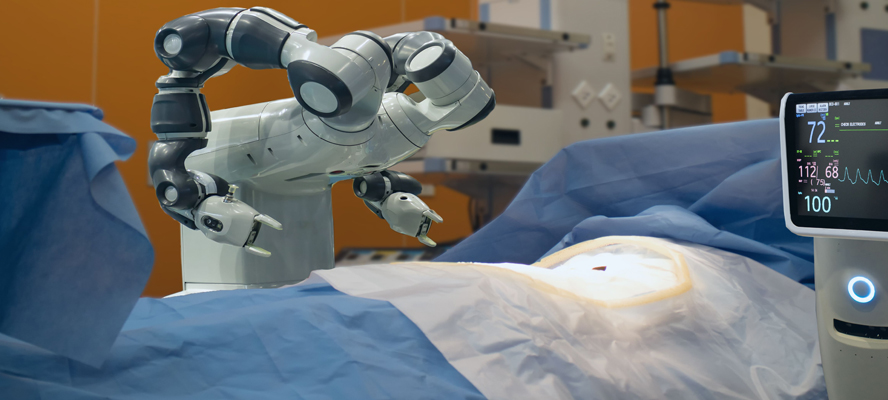
\includegraphics[scale=0.2]{rob.jpg}
 \\
Robots were used medically for the first time in 1985. Since then, their role has expanded in this sector. The revenue generated in this segment is expected to reach USD 2.08 billion in 2021. Robots are mostly used in surgeries and to some extent in procedures such as laparoscopy, neurosurgery, orthopedic surgery, emergency response, and minimally invasive operations. The technology also has wearables such as robotic prostheses or exoskeletons that help with mobility issues in those suffering from missing or paralyzed limbs. Additionally, robotics are deployed for mundane tasks like restocking, disinfecting, cleaning, etc. Robots also gaining popularity as companions for the elderly or child patients.
\subsection*{3D Bioprinting}
 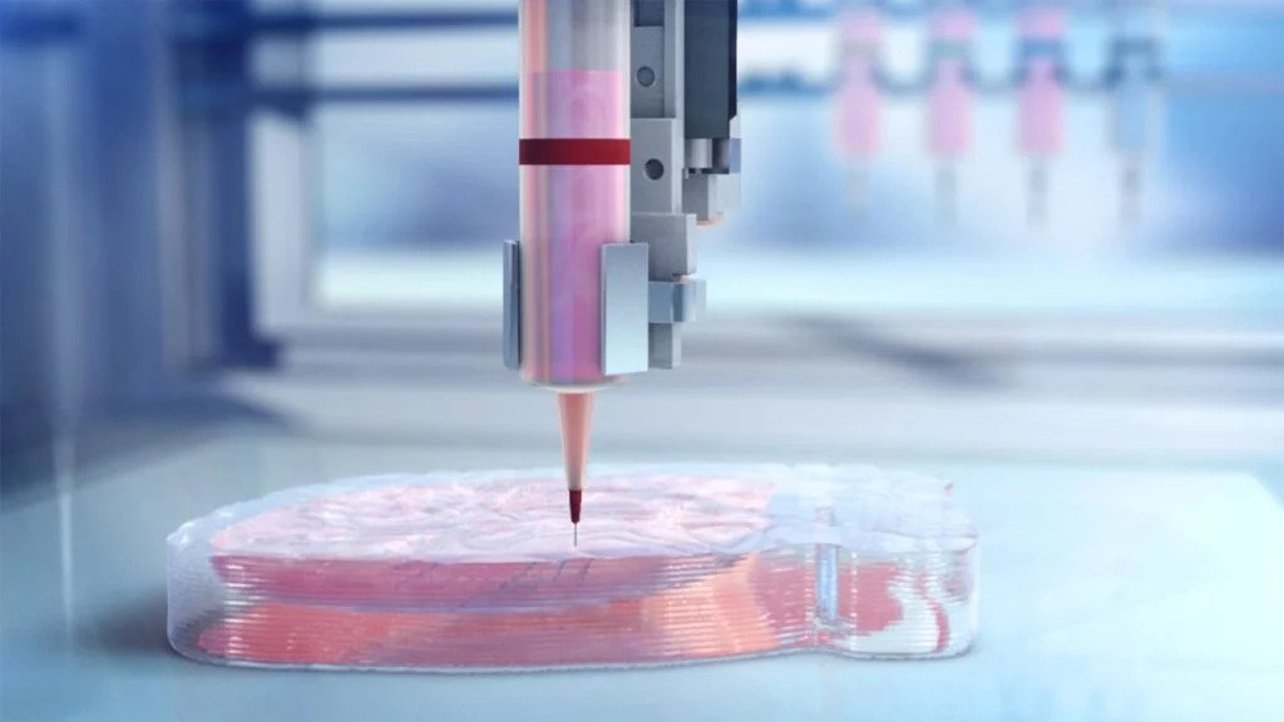
\includegraphics[scale=0.15]{print.jpg }
 \\
Another technological innovation for the healthcare space is 3D bioprinting. The global bioprinting market could have investments of almost USD 1.8 billion by 2027. With the help of DNA analysis, bio-printing can regenerate and replace several body parts, bones, and tissue. Recently, a research team developed a method to 3D-print living skin and blood vessels. This is a great breakthrough for skin grafts for burn victims. 3D-print prosthetics are also a boon for patients with missing limbs.
\subsection*{Nano-Technology}
 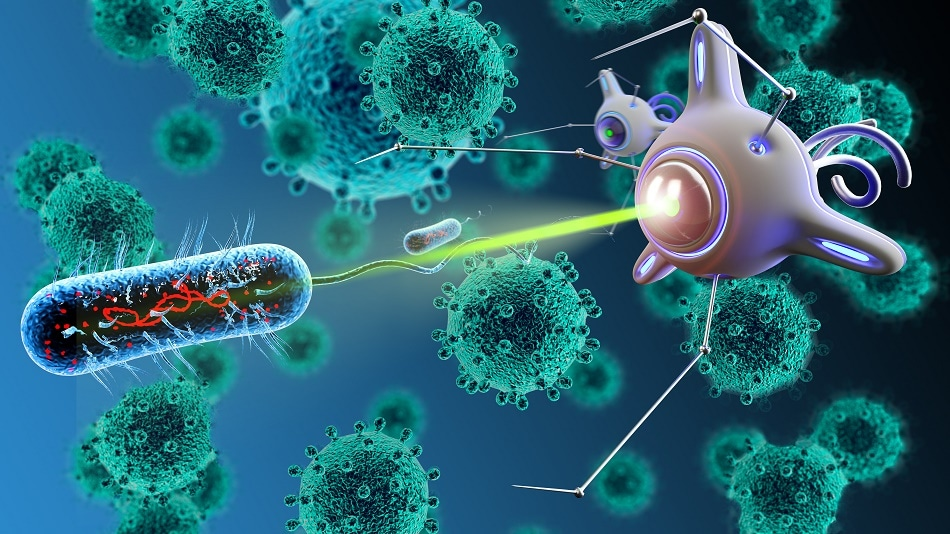
\includegraphics[scale=0.2]{nano.jpg }
 \\
Nanotechnology for the healthcare space has been under development for a long time now. It studies molecular structure to develop precise devices and medicines. Some of developments using nanotechnology include nanorobots and nanomedicines. In 2018, an electronic pill was developed using nanotechnology; the pill can be controlled after release in the patient’s body to relay diagnostic details or to release drugs in a specific section of the body. Currently, the technology is used to make smart patches that can monitor wounds and stimulate rapid healing. Most of this application is still under research.


\enddocument